% Options for packages loaded elsewhere
\PassOptionsToPackage{unicode}{hyperref}
\PassOptionsToPackage{hyphens}{url}
%
\documentclass[
]{article}
\usepackage{amsmath,amssymb}
\usepackage{lmodern}
\usepackage{iftex}
\ifPDFTeX
  \usepackage[T1]{fontenc}
  \usepackage[utf8]{inputenc}
  \usepackage{textcomp} % provide euro and other symbols
\else % if luatex or xetex
  \usepackage{unicode-math}
  \defaultfontfeatures{Scale=MatchLowercase}
  \defaultfontfeatures[\rmfamily]{Ligatures=TeX,Scale=1}
\fi
% Use upquote if available, for straight quotes in verbatim environments
\IfFileExists{upquote.sty}{\usepackage{upquote}}{}
\IfFileExists{microtype.sty}{% use microtype if available
  \usepackage[]{microtype}
  \UseMicrotypeSet[protrusion]{basicmath} % disable protrusion for tt fonts
}{}
\makeatletter
\@ifundefined{KOMAClassName}{% if non-KOMA class
  \IfFileExists{parskip.sty}{%
    \usepackage{parskip}
  }{% else
    \setlength{\parindent}{0pt}
    \setlength{\parskip}{6pt plus 2pt minus 1pt}}
}{% if KOMA class
  \KOMAoptions{parskip=half}}
\makeatother
\usepackage{xcolor}
\usepackage[margin=1in]{geometry}
\usepackage{graphicx}
\makeatletter
\def\maxwidth{\ifdim\Gin@nat@width>\linewidth\linewidth\else\Gin@nat@width\fi}
\def\maxheight{\ifdim\Gin@nat@height>\textheight\textheight\else\Gin@nat@height\fi}
\makeatother
% Scale images if necessary, so that they will not overflow the page
% margins by default, and it is still possible to overwrite the defaults
% using explicit options in \includegraphics[width, height, ...]{}
\setkeys{Gin}{width=\maxwidth,height=\maxheight,keepaspectratio}
% Set default figure placement to htbp
\makeatletter
\def\fps@figure{htbp}
\makeatother
\setlength{\emergencystretch}{3em} % prevent overfull lines
\providecommand{\tightlist}{%
  \setlength{\itemsep}{0pt}\setlength{\parskip}{0pt}}
\setcounter{secnumdepth}{-\maxdimen} % remove section numbering
\usepackage{multicol}
\usepackage{graphicx}
\ifLuaTeX
  \usepackage{selnolig}  % disable illegal ligatures
\fi
\IfFileExists{bookmark.sty}{\usepackage{bookmark}}{\usepackage{hyperref}}
\IfFileExists{xurl.sty}{\usepackage{xurl}}{} % add URL line breaks if available
\urlstyle{same} % disable monospaced font for URLs
\hypersetup{
  pdftitle={OvRSeq Analysis Report for TCGA-04-1331},
  hidelinks,
  pdfcreator={LaTeX via pandoc}}

\title{OvRSeq Analysis Report for TCGA-04-1331}
\author{}
\date{\vspace{-2.5em}2023-11-25}

\begin{document}
\maketitle

\hypertarget{ovrseq-analysis-results-for-patient-tcga-04-1331}{%
\subsection{OvRSeq Analysis Results for Patient:
TCGA-04-1331}\label{ovrseq-analysis-results-for-patient-tcga-04-1331}}

The report starts with a Vulnerability Map highlighting HGSOC aspects,
including BRCAness Status, Infiltration Status, and Tumor Molecular
Subtypes, setting the stage for a personalized molecular analysis.

\begin{multicols}{2}

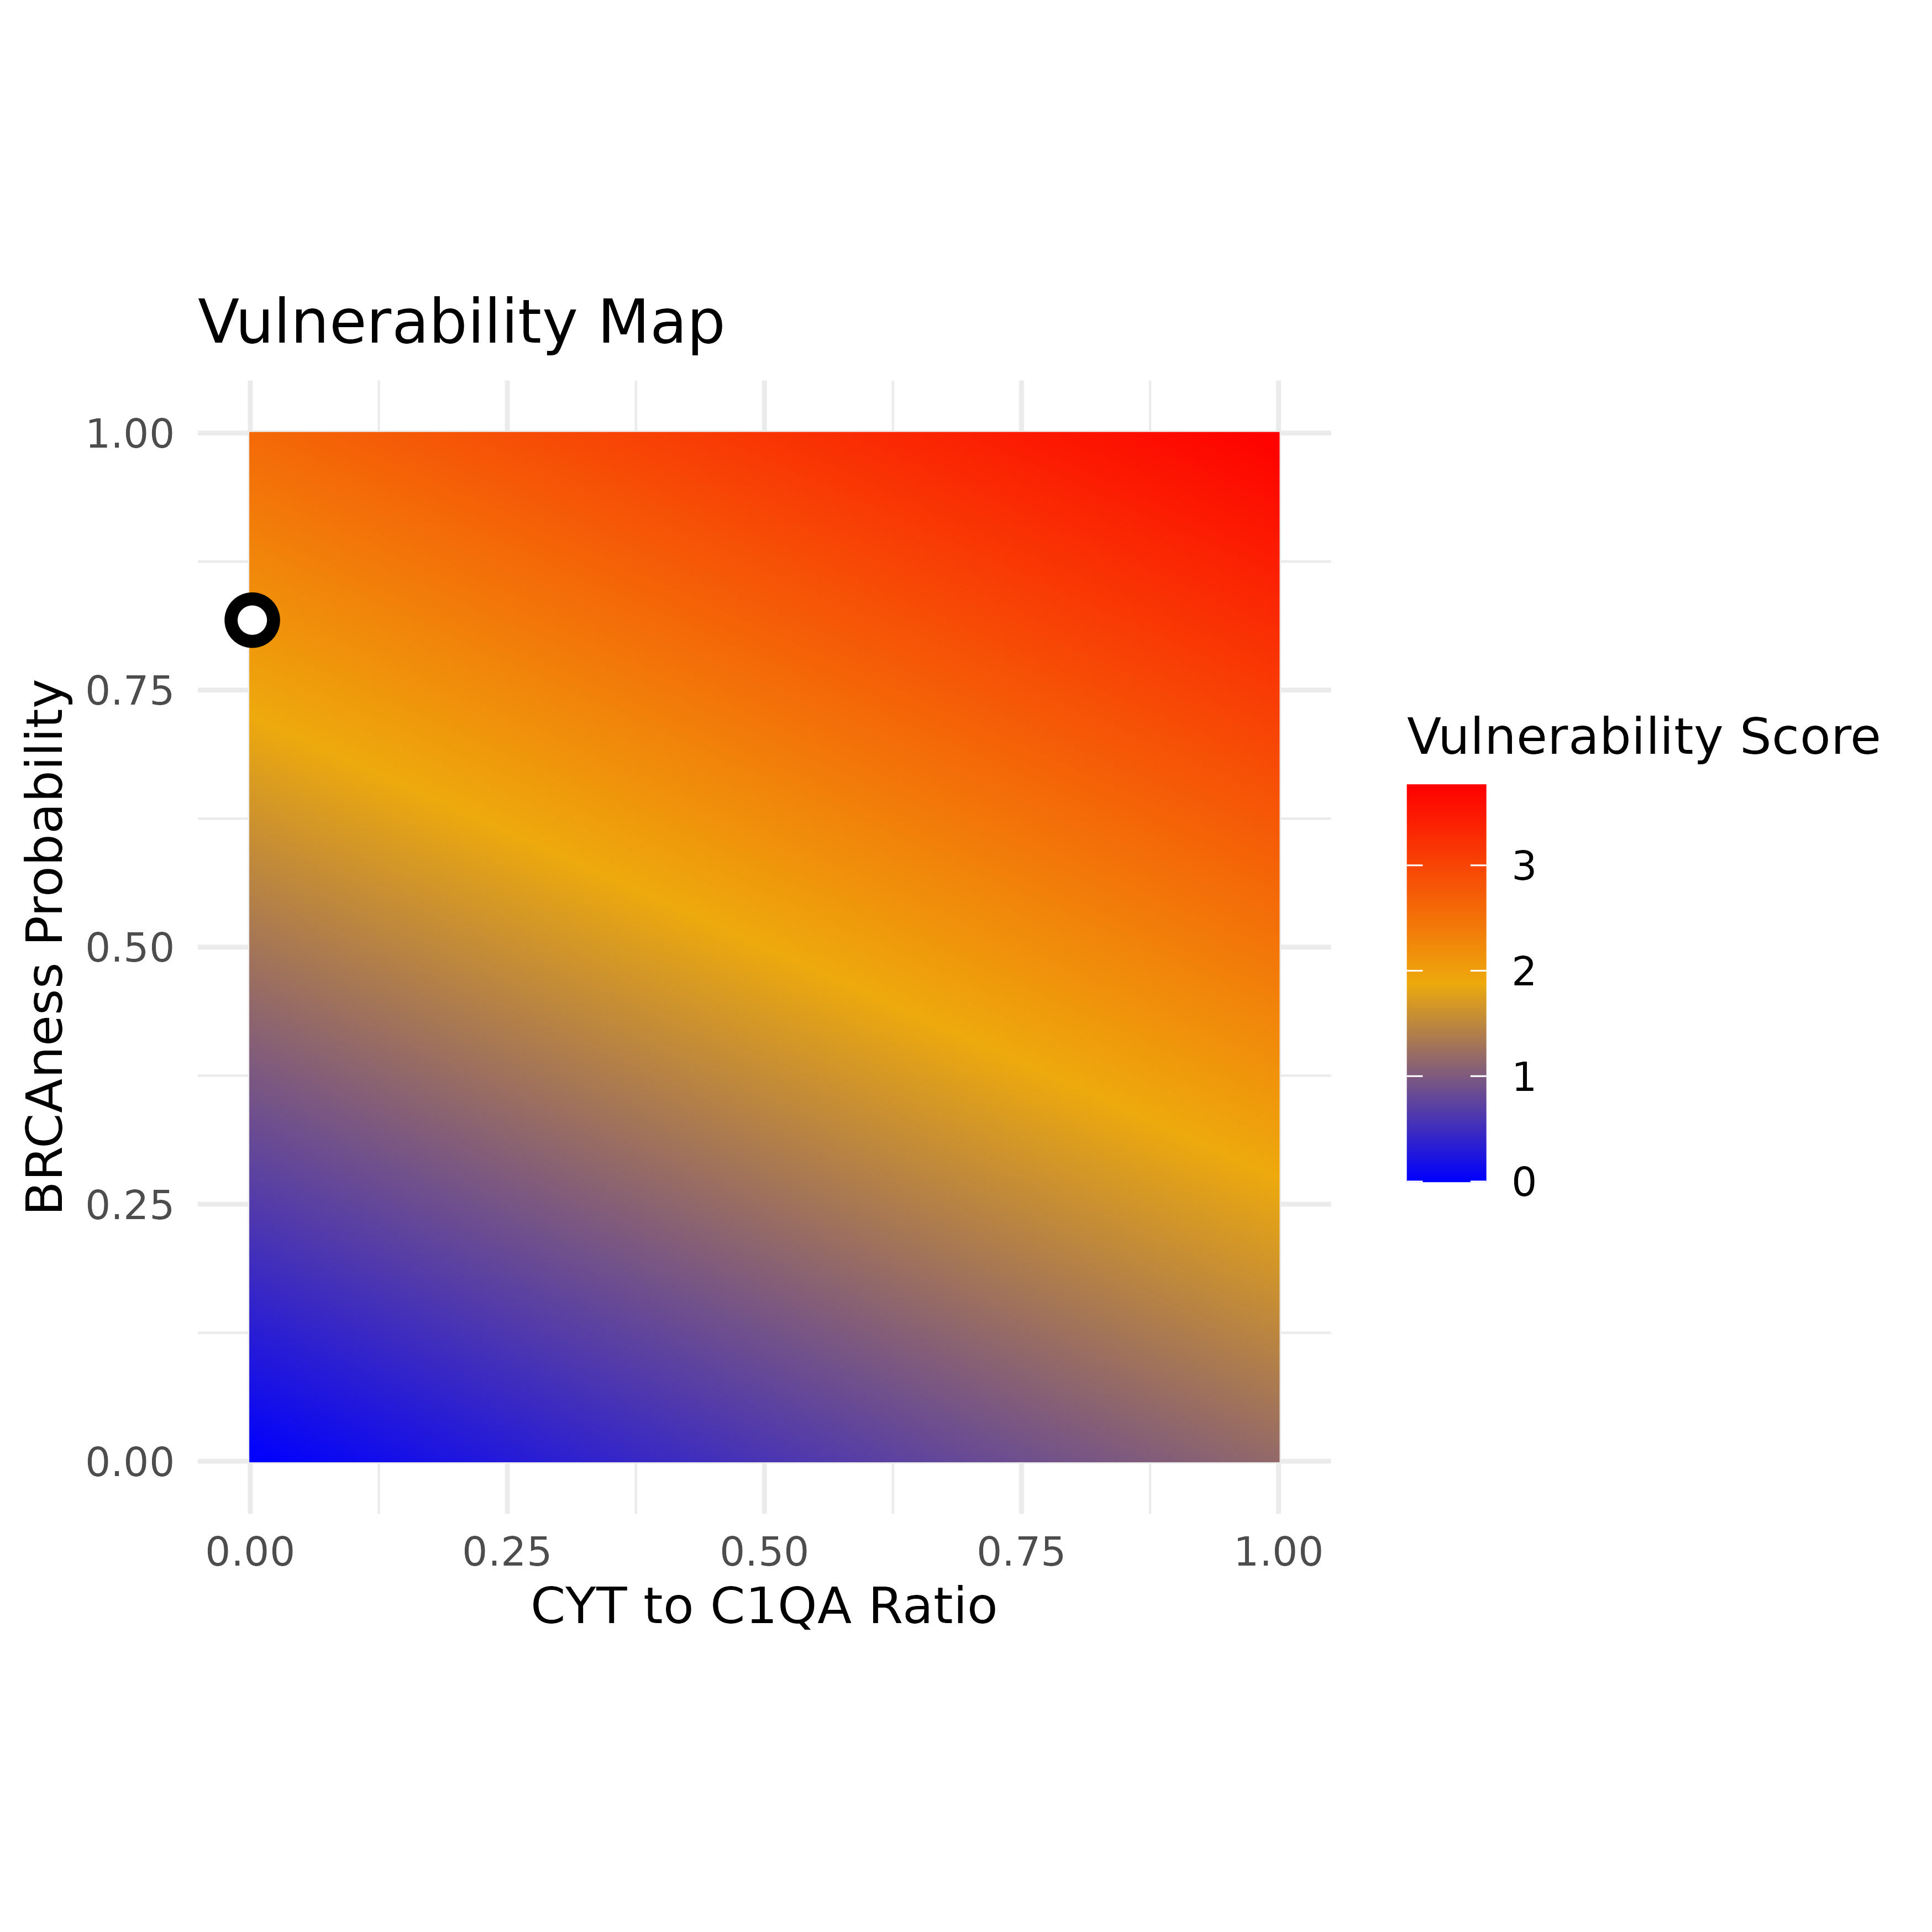
\includegraphics{./p1.jpeg}

\columnbreak

\textbf{Patient Values}

\begin{tabular}{cc}
\hline
Feature & Value \\
\hline
BRCAness Status & 1 (0.818) \\
Infiltration Status & Desert \\
Molecular Subtypes & PRO consensus \\
BRCAness immunotype & other \\
Vulnerability Score & 2.389 \\
Immuno Phenoscore & 1 \\
CYT to C1QA Ratio & 0.002 \\
Angiogenesis Score &  \\
\hline
\end{tabular}

\end{multicols}

\textbf{Molecular markers and TCGA-OV Reference Values}

This report section compares the patient's molecular markers with TCGA
interquartile ranges (IQR). The table includes key markers like Immuno
Phenoscore and CYT to C1QA ratio, crucial for personalized cancer
profiling and treatment.

\begin{multicols}{2}

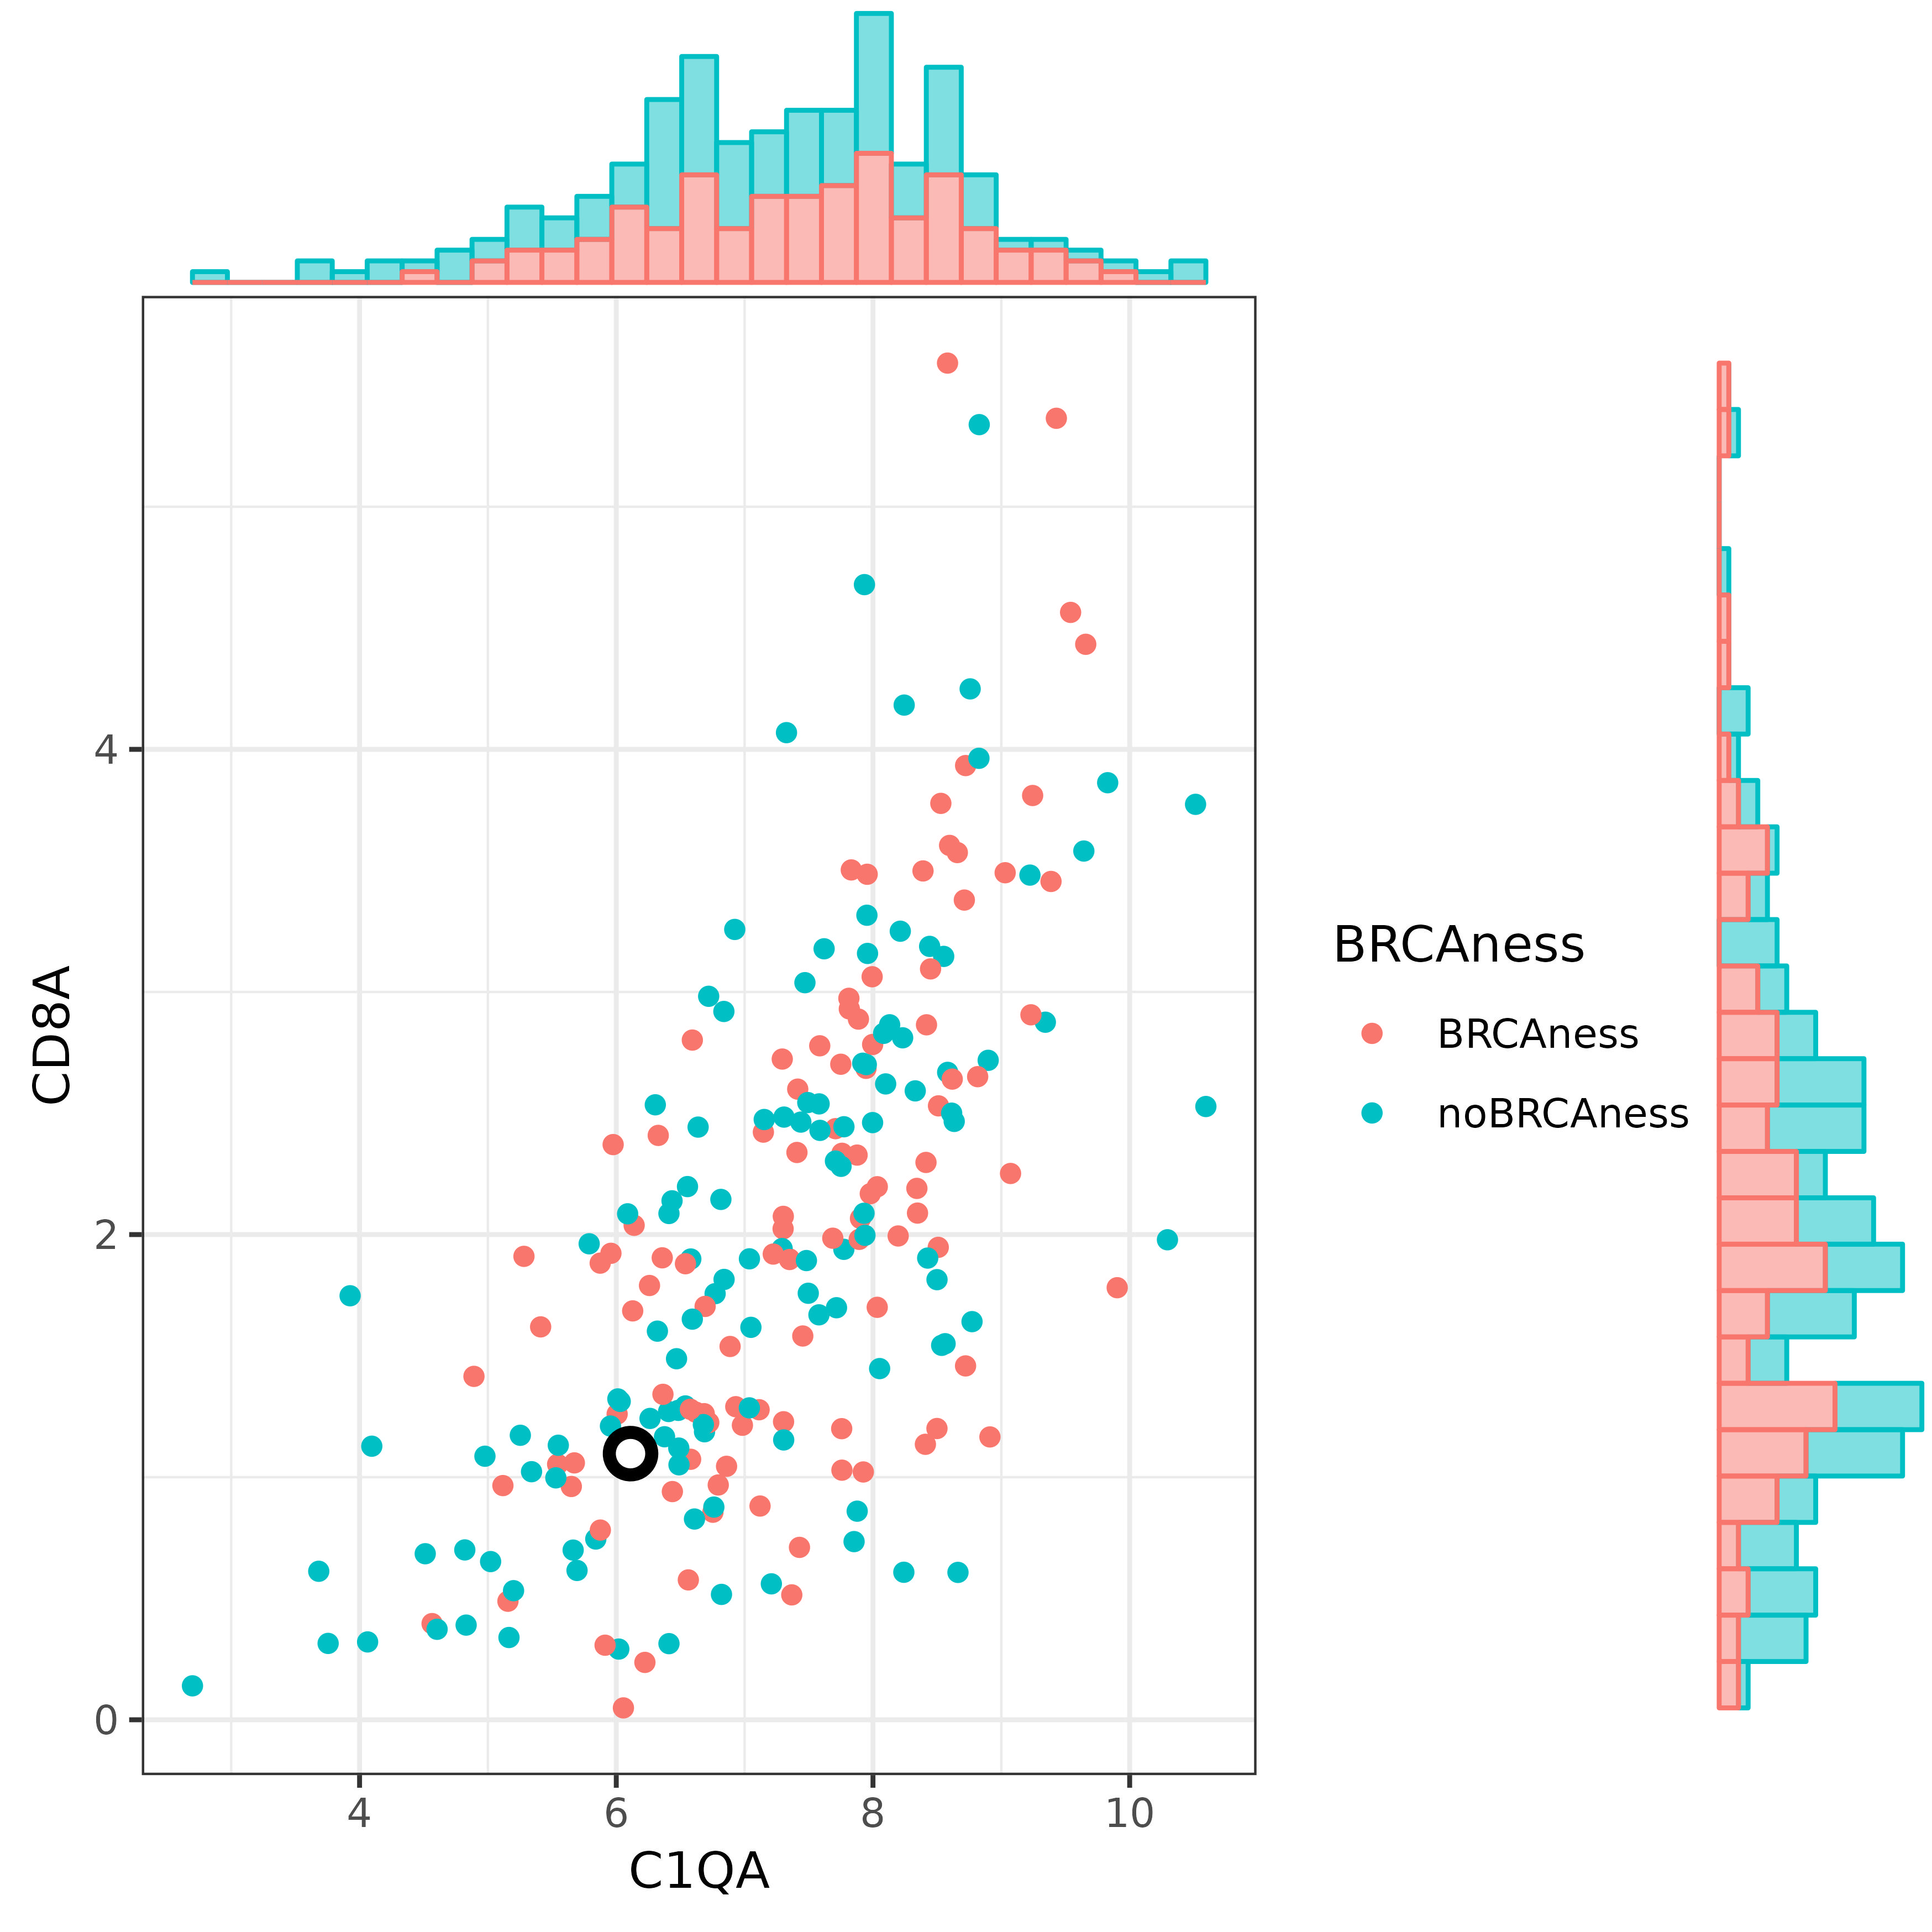
\includegraphics{./p2.jpeg}

\columnbreak

\begin{tabular}{lll}
\hline
Feature & Patient Value & TCGA IQR \\
\hline
CD274 & 1.21 & 1.325 (0.874-1.859) \\
GZMB & 2.149 & 2.548 (1.625-3.511) \\
PRF1 & 0.627 & 1.731 (1.152-2.505) \\
C1QA & 6.111 & 7.35 (6.411-8.18) \\
CD8A & 1.097 & 1.904 (1.168-2.648) \\
IDO1 & 4.113 & 4.161 (2.802-5.446) \\
FOXP3 & 1.748 & 1.938 (1.318-2.521) \\
TREM2 & 3.606 & 4.83 (3.761-5.638) \\
STAT1 & 7.266 & 7.015 (6.207-7.551) \\
HLA-DRA & 5.214 & 7.262 (6.298-8.001) \\
CXCL10 & 4.719 & 6.379 (5.032-7.539) \\
\hline
\end{tabular}

\end{multicols}

\end{document}
